\documentclass[a4paper, 11pt]{article}
\usepackage{verbatim} 
\usepackage{amsmath}
\usepackage{amsfonts}
\usepackage{amssymb}
\usepackage{amsthm}
\usepackage{caratula}
\usepackage{listings}
\usepackage[utf8]{inputenc}
\usepackage[spanish, activeacute]{babel}
\usepackage[usenames,dvipsnames]{color}
\usepackage[width=15.5cm, left=3cm, top=2.5cm, height= 24.5cm]{geometry}
\usepackage{graphicx}
%\usepackage{subcaption}
\usepackage[all]{xy}
\usepackage{multicol}
\usepackage{subfig}
\usepackage{algorithm}
\usepackage{algorithmic}
\usepackage{cancel}
\usepackage{array}
\usepackage{float}
\usepackage{xcolor}
\usepackage{color,hyperref}
\setcounter{secnumdepth}{3} %%agrego subsubsection
\usepackage[nottoc,notlot,notlof]{tocbibind}

\newtheorem{lema}{Lema}
\newtheorem{teorema}{Teorema}
\newtheorem{corolario}{Corolario}
\newtheorem*{correctitud}{Correctitud del algoritmo}
\newtheorem*{notacion}{Notación}

\lstset{basicstyle=\small\ttfamily, breaklines=true, breakatwhitespace=true}
\lstset{numbers=left, numberstyle=\scriptsize}
\lstset{
     literate=%
         {á}{{\'a}}1
         {í}{{\'i}}1
         {é}{{\'e}}1
         {ý}{{\'y}}1
         {ú}{{\'u}}1
         {ó}{{\'o}}1
         {ě}{{\v{e}}}1
         {š}{{\v{s}}}1
         {č}{{\v{c}}}1
         {ř}{{\v{r}}}1
         {ž}{{\v{z}}}1
         {ď}{{\v{d}}}1
         {ť}{{\v{t}}}1
         {ñ}{{\~n}}1                
         {ů}{{\r{u}}}1
         {Á}{{\'A}}1
         {Í}{{\'I}}1
         {É}{{\'E}}1
         {Ý}{{\'Y}}1
         {Ú}{{\'U}}1
         {Ó}{{\'O}}1
         {Ě}{{\v{E}}}1
         {Š}{{\v{S}}}1
         {Č}{{\v{C}}}1
         {Ř}{{\v{R}}}1
         {Ž}{{\v{Z}}}1
         {Ď}{{\v{D}}}1
         {Ť}{{\v{T}}}1
         {Ň}{{\v{N}}}1                
         {Ů}{{\r{U}}}1    
}


%%%%%%%%%%%%%% ALGUNAS MACROS %%%%%%%%%%%%%%
% For \url{SOME_URL}, links SOME_URL to the url SOME_URL
\providecommand*\url[1]{\href{#1}{#1}}

\setlength{\parskip}{10pt plus 1pt minus 1pt}
\usepackage{tikz}
\def\checkmark{\tikz\fill[scale=0.4](0,.35) -- (.25,0) -- (1,.7) -- (.25,.15) -- cycle;}

% Same as above, but pretty-prints SOME_URL in teletype fixed-width font
\renewcommand*\url[1]{\href{#1}{\texttt{#1}}}

% Comando para poner el simbolo de Reales
\newcommand{\real}{\hbox{\bf R}}

\providecommand*\code[1]{\texttt{#1}}

%uso: \ponerGrafico{file}{caption}{scale}{label}
\newcommand{\ponerGrafico}[4]
{\begin{figure}[H]
	\centering
	\subfloat{\includegraphics[scale=#3]{#1}}
	\caption{#2} \label{fig:#4}
\end{figure}
}

\renewcommand{\algorithmiccomment}[1]{\hfill #1}

%%%%%%%%%%%%%%%%%%%%%%%%%%%%%%%%%%%%%%%%%%%%

\materia{Algoritmos y Estructuras de Datos III}

\titulo{Trabajo práctico 3}
%\fecha{fecha de entrega}
%\grupo{Nro grupo}
\integrante{Sebastián Fernández Ledesma}{392/06}{sfernandezledesma@gmail.com}
\integrante{Fernando Gasperi Jabalera}{56/09}{fgasperijabalera@gmail.com}
\integrante{Maximiliano Wortman}{892/10}{maxifwortman@gmail.com}
\integrante{Santiago Camacho}{110/09}{santicamacho90@gmail.com}


%\include{templates}

\begin{document}
\pagestyle{myheadings}
\maketitle
%\markboth{Nombre materia}{Nombre TP}

\thispagestyle{empty}
\tableofcontents

%\setcounter{section}{-1}
\newpage
\section{Ejercicio 1}

\begin{displaymath}
	\sum_0^{\infty}laposta de 
\end{displaymath}

\section{Algoritmo exacto}

\subsection{Descripción del algoritmo}
El algoritmo utilizado para obtener la $k$-PMP de un grafo $G$ consiste en construir 
todas las posibles soluciones de manera ordenada para mediante backtracking.
Veamos qué contiene el conjunto de soluciones posibles $S$ asociado a un grafo $G = (V, E)$.
Sea $P_V$ el conjunto con todas las particiones posibles del conjunto $V$:
\begin{displaymath}
  S = \left\{p \quad | \quad p \in P_V \land \left\vert{p}\right\vert \leq k\right\}
\end{displaymath}
Todas las particiones de un conjunto de $n$ elementos se pueden obtener recursivamente. Si contamos
con todas las particiones de $i$ elementos, denominaremos $S_i$ al conjunto que contiene a todas las
particiones de $i$ elementos, entonces podemos generar todas las particiones de $i+1$ elementos simplemente 
tomando cada una de las particiones pertenecientes a $S_i$ y agregando el elemento $i+1$ a cada uno 
de sus subconjuntos. Describimos este procedimiento con un pequeño pseudocódigo:

\begin{algorithm}[H]
\begin{algorithmic}
\caption{Particiones}
  \STATE $S_{i+1}\gets \emptyset$
  \WHILE {$S_i \neq \emptyset$}
    \STATE $s\gets$ sacarUno($S_i$)
    \FOR {$j \gets 0...\left\vert{s}\right\vert$}
      \STATE $nuevoSubconjunto \gets $ dameIesimo($j$, $s$)
      \STATE $nuevoSubconjunto \cup e_{i+1}$
      \STATE $S_{i+1} \cup \left\{ s \setminus \text{dameIesimo(}j\text{, }s\text{)} \cup nuevoSubconjunto \right\}$
    \ENDFOR
  \ENDWHILE
\end{algorithmic}
\end{algorithm}

Se puede ver fácilmente que con este procedimiento efectivamente consideramos todas las particiones
posibles que se pueden obtener con los $n$ vértices de $V$. Sin embargo, estamos considerando muchas
particiones que no es necesario tener en cuenta. Por ejemplo, aquellas que tengan una cantidad de
subconjuntos mayor a $k$.

\subsection{Podas y estrategias}
%\begin{lema}
%\label{lema_ej2}
%acá va el enunciado del lema
%\end{lema}
%\begin{proof}
%  Acá va la demostración.
%\end{proof}

Las podas que le agregamos a nuestro backtracking para reducir el árbol de soluciones son:
\begin{enumerate}
  \item no consideraremos particiones que tengan más de $k$ subconjuntos. Una vez que tenemos
    $k$ subconjuntos en la solución actual no agregamos más ya que la solución no puede tener
    más de $k$ subconjuntos. El costo de esta poda es $O(1)$ porque sólo requiere una comparación
    de tipos primitivos.

  \item no considerar particiones que utilicen menos de $k$ subconjuntos. Si estamos
    buscando la $k$-PMP de $G$, llamémosla $P_{min}$ y la misma utiliza menos de $k$ subconjuntos 
    $|P_{min}| < k$ entonces su peso total necesariamente es nulo $\omega(P_{min}) = 0$ ya que si
    hubiera algún subconjunto $s$ con peso mayor 0 eso indicaría que existe alguna arista $e = (v, u)$ intra-partición
    en ese subconjunto con peso mayor a 0. Por lo tanto, si tomamos a $v$ uno de los extremos de esa
    arista y lo pasamos a un subconjunto $s'$ vacío entonces obtendríamos una nueva partición con un peso
    estrictamente menor al de la mínima lo cual es absurdo.
    En el algoritmo esto se ve reflejado cuando la cantidad de subconjuntos no utilizados es igual a la cantidad 
    de nodos que nos quedan por ubicar $|P_{actual}|-k = |nodosRestantes|$. En ese caso lo que hacemos es agregar los $|nodosRestantes|$
    a cada uno de los subconjuntos todavía no utilizados ya que cualquier partición $P'$ que agregue alguno
    de los $nodosRestantes$ a uno de los subconjuntos ya utilizados necesariamente cumple que 
    $\omega(P') \geq \omega(P_{actual})$ porque $P_{actual}$ no va a tener más aristas intra-partición
    y agregando nodos a conjuntos ya utilizados puede que agreguemos aristas intra-partición o no.
    Esta poda también tiene costo $O(1)$ porque sólo necesita que se comparen la cantidad de subconjuntos
    vacíos con la cantidad de nodos restantes. Ambos valores son conocidos en todo momento del algoritmo.

  \item inicializamos $pesoMinimo = +\infty$ y cada vez que encontramos una nueva partición que incluye a todos
    los nodos comparamos su peso con el de $pesoMinimo$ si su peso es menor entonces actualizamos $pesoMinimo$
    y la partición mínima encontrada hasta el momento. De esta forma siempre sabemos cuál es el peso de la mejor 
    solución obtenida hasta el momento. Entonces, cada vez que vamos a agregar un nodo a un subconjunto comparamos
    cuál sería el peso total de la nueva partición generada con el de la mínima actual. Si resulta ser mayor o igual
    no hacemos la llamada recursiva porque sabemos que agregar nodos a la partición sólo puede incrementar el peso
    de total de la partición porque todas las aristas tienen pesos positivos. Esta poda tiene costo $O(1)$ ya
    que también implica la comparación de dos valores ya conocidos: el peso total de la partición actual
    y el peso de la mínima obtenida hasta el momento.

  \item si ya existen elementos en los $k$ subconjuntos, es decir no restan subconjuntos vacíos,
    calculamos el peso que aportaría a la partición agregar cada uno de los nodos restantes al 
    subconjunto que menos peso agregue. Es decir, calculo el mínimo peso
    que pueden llegar a sumar a la partición actual los $i$ nodos restantes. Si la suma de todos los pesos 
    más el peso actual es mayor al mínimo obtenido hasta el momento dejo de recorrer esa rama. El costo 
    de esta poda es $O(n^2)$ porque por cada nodo restante $(n-i)$ tengo que recorrer $i$. El máximo posible
    es $\frac{n^2}{4}$ que es del orden de $n^2$. 
\end{enumerate}

\subsection{Complejidad temporal}
Para analizar la complejidad temporal del algoritmo veremos por un lado el costo que pagamos en cada llamada recursiva
y por otro la cantidad de llamadas recursivas que realizamos. La función auxiliar utilizada en cada llamada recursiva
es $calcularPesoEnSubconjunto$. Esta función es llamada una vez por cada subconjunto, por lo tanto,
cuando estamos agregando el nodo $v_i$ tiene una complejidad amortizada de $O(i)$ ya que la cantidad
total de nodos en todos los subconjuntos es $i$ y no recorremos subconjuntos vacíos. La cantidad de llamadas recursivas
es igual a la cantidad de particiones de $i$ elementos en $j$ subconjuntos con $1 \leq i \leq n$ y $1 \leq j \leq k$. Ya que
como vimos antes generamos todas las particiones de los $n$ nodos en $k$ subconjuntos diferentes de forma recursiva
utilizando en el paso $i$ las particiones de $i-1$ elementos y agregamos el elemento $i$ en cada uno de los subconjuntos
de cada una de las particiones. Este objeto combinatorio, cantidad de formas de ubicar $n$ objetos en $k$ subconjuntos
sin dejar subconjuntos vacíos, está representado por los números de Stirling de segunda especie:
\begin{displaymath}
  S(n, k) = \left\{\begin{matrix} n \\ k \end{matrix}\right\} = \frac{1}{k!}\sum_{j=0}^k (-1)^{j}{k \choose j} (k-j)^n
\end{displaymath}
aquí presentamos su fórmula exacta la cual se vale del principio de inclusión-exclusión para resolver el conteo.
Una cota superior conocida para la función $S(n ,k)$ es:
\begin{displaymath}
  S(n, k) \leq \frac{1}{2}{n \choose k} k^{n-k}
\end{displaymath}
Sin embargo, este valor sólo representa las hojas de nuestro árbol de backtracking ya que al nosotros generarlas
recursivamente primero generamos $S(i, j)$ con $1 \leq i \leq n$ y $1 \leq j \leq k$. Por lo tanto las
llamadas recursivas totales son:
\begin{displaymath}
  \sum_{i=0}^n\sum_{j=0}^k S(i, j) \leq \sum_{i=0}^n\sum_{j=0}^k \frac{1}{2}{i \choose j} j^{i-j}
\end{displaymath}
La cota de complejidad resulta ser:
\begin{displaymath}
  O(\sum_{i=0}^n\sum_{j=0}^k \frac{1}{2}{i \choose j} j^{i-j}i)
\end{displaymath}
porque le agregamos el costo de calcular el peso en cada uno de los subconjuntos. Ésta cota se corresponde
con la complejidad del algoritmo utilizando las podas 1 y 2 porque no consideramos subconjuntos vacíos y
tampoco consideramos más de $k$ subconjuntos. La complejidad temporal del algoritmo sin podas es equivalente
a la de \textit{Biohazard} ya que consideramos todas las particiones de un conjunto de $n$ elementos, en este caso
los nodos y recordamos que era:
\begin{displaymath}
  O(\sum_{i=0}^ni!)
\end{displaymath}

\subsection{Experimentación}
El objetivo de esta experimentación es revisar las cotas de complejidad obtenidas a través del análisis teórico
a la luz de resultados empíricos y comparar las diferentes podas para ver cuáles son más eficientes y si 
resulta beneficioso componerlas. Por composición de podas nos referimos a aplicar más de una, lo cual no necesariamente
es mejor que aplicar sólo una ya que quizás realizan podas parecidas duplicando el trabajo para podar lo mismo.
En primer lugar, ejecutamos el algoritmo sin podas para instancias de hasta 11 nodos, ya que con más nodos
tomaba demasiado tiempo, y dividimos el tiempo por $\sum_{i=0}^ni!$ que era la cota que habíamos
obtenido para el algoritmo sin podas. Esperamos que la curva se asemeje a una recta constante. Cada instancia
la corrimos 10 veces y nos quedamos con el tiempo mínimo de las 10 corridas. Para cada $1 \leq n \leq 12$ corrimos
100 instancias generadas pseudoaleatoriamente y nos quedamos con el promedio de las 100:
\begin{center}
  \begin{tabular}{ c | c | c | c | c | c}
    $n$ & sin podas & $k$ subconjuntos & mínimo peso & hay mejora & compuestas \tabularnewline \hline
    3 & 86 & 74 & 70 & 74 & 64 \tabularnewline \hline
    4 & 199 & 148 & 125 & 130 & 118 \tabularnewline \hline
    5 & 525 & 276 & 204 & 203 & 183 \tabularnewline \hline
    6 & 1760 & 557 & 372 & 359 & 324 \tabularnewline \hline 
    7 & 6906 & 1096 & 651 & 561 & 516 \tabularnewline \hline 
    8 & 30305 & 2177 & 1175 & 936 & 886 \tabularnewline \hline
    9 & 149877 & 21016 & 3240 & 5034 & 2133 \tabularnewline \hline
    10 & 819763 & 62888 & 7192 & 10064 & 4026 \tabularnewline \hline
    11 & 4561726 & 160775 & 13322 & 17324 & 6527
  \end{tabular}
\end{center}
Donde:
\begin{description}
  \item[sin podas] backtracking sin podas.
  \item[$k$ subconjuntos] aplicamos simultáneamente las podas de no seguir agregando nuevos subconjuntos si ya tenemos
    $k$ y no generar particiones con menos de $k$ subconjuntos.
  \item[hay mejora] se refiere a la poda en la que evaluamos si colocando a todos los nodos que restan en sus respectivos
    subconjuntos en los que aportan el mínimo peso posible se mejoraría el mínimo peso obtenido hasta el momento.
  \item[compuestas] se efectuaron las 4 podas simultáneamente.
\end{description}

En esta primer tabla presentamos los tiempos obtenidos en microsegundos ($\mu s$). Decidimos presentar estos resultados
en forma de tabla y no como un gráfico ya que al sólo poder comparar con pocos valores de $n$, por las restricciones de
tiempo impuestas por la variante del backtracking \textit{sin podas}, los gráficos reflejan de forma pobre las relaciones
entre las diferentes podas. Ordenándolas por su performance en estas instancias obtenemos:

\begin{displaymath}
  compuestas < minimo\text{ }peso < hay\text{ }mejora << k\text{ }subconjuntos << sin\text{ }podas
\end{displaymath}

Los mayores saltos los encontramos entre \textit{sin podas} y el resto de las podas y entre la poda \textit{k subconjuntos}
y el resto. Una posible explicación al segundo salto considerado es que la restricción de sólo contar con $k$ subconjutos
queda implícita en el resto de las podas ya que, como vimos en la sección en la que analizamos cada una por separado,
necesariamente una solución en la mayoría de los casos cuenta con exactamente $k$ subconjuntos y no con menos. Además, 
podemos ver que la composición de podas obtuvo la mejor performance, este es un buen indicio de que las podas mejoran
su performance si se ejecutan en simultáneo. Sin embargo, es necesario realizar comparaciones de a pares para ver 
si todas realmente mejoran entre sí. Por ejemplo, tomamos \textit{mínimo peso} y \textit{hay mejora}, las corremos 
en simultáneo y por separado. Luego, comparamos los tiempos para ver si efectivamente se mejoran entre sí. Este
procedimiento se debería realizar para todos los pares posibles para extraer de alguna forma las podas que de alguna
forma podan de manera más disjunta posible, es decir que las ramas que podan prácticamente no se superponen.

\begin{center}
  \begin{tabular}{ c | c | c | c | c | c}
    $n$ & sin podas$ / \sum_{i=0}^ni!$ & k subconjuntos (\%) & compuestas (\%) \tabularnewline \hline
    3 & 9 & 86 & 74 \tabularnewline \hline
    4 & 8 & 74 & 59 \tabularnewline \hline
    5 & 3 & 52 & 34 \tabularnewline \hline
    6 & 2 & 31 & 18 \tabularnewline \hline 
    7 & 1.16 & 15 & 7 \tabularnewline \hline 
    8 & 0.6 & 7 & 3 \tabularnewline \hline
    9 & 0.3 & 14 & 1 \tabularnewline \hline
    10 & 0.2  & 7 & 0.5 \tabularnewline \hline
    11 & 0.1 & 3 & 0.1
  \end{tabular}
\end{center}

En esta segunda tabla, en la primer columna tenemos los tiempos de \textit{sin podas} divididos por la cota
de complejidad obtenida. Vemos que los valores decrecen pero de forma muy lenta. Con tan pocos valores
no estamos seguros si esto se debe a que la cota de complejidad es demasiado holgada o simplemente es un comportamiento
que sólo se observa en estos primeros valores de $n$ y luego se mantiene constante. Para obtener más información es necesario
correr el algoritmo para más valores de $n$. En la segunda y tercer columna tenemos el porcentaje del tiempo entre el tomado
por una cota con respecto al sin podas:
\begin{displaymath}
  \frac{t(con\text{ }poda) \times 100}{t(sin\text{ }podas)}
\end{displaymath}
el objetivo de presentar esta información es doble. Por un lado, queríamos ver la gran mejora que puede representar
aplicar aunque sea sólo una cota con respecto a correr el algoritmo sin ellas y por otro ver más claramente como diferentes
podas tiene mejor performance que otras. En este caso en particular elegimos comparar \textit{compuestas} porque nos parece
que lo más interesante es generar más podas e ir comparandolas con las ya obtenidas de a pares como ya explicamos. Si 
la comparación es favorable querrá decir que agregarla a nuestro set de podas redundará en una mejora de la performance
y por lo tanto habremos enriquecido nuestra poda compuesta.

\section{Ejercicio 3}

Definimos el peso de un nodo como la suma de los pesos de las aristas que inciden sobre él. La idea de la heurística golosa constructiva es entonces ``aislar'' a los nodos más pesados, bajo la premisa de que éstos son los más problemáticos y deben ser los primeros en procesarse.

Lo que se hace en un principio es agarrar el nodo más pesado, y agregarlo a un conjunto. Después, se busca el nodo más pesado de los no asignados, y se pone en el mejor conjunto disponible. El criterio para elegir a un conjunto es el peso del nodo en ese conjunto. Y así siguiendo hasta que no haya mas nodos. El pseudocódigo es:
\begin{algorithm}[H]
\begin{algorithmic}[1]
\caption{HeuristicaGolosaConstructiva(Grafo G, nat k)}
\STATE Vector$<$Conjunto$<$Nat$>>$ conjuntos(k, vacío)
\STATE Vector$<$Nat$>$ nodosOrdenados $\leftarrow$ OrdenarNodosPorPesoEnGrafoDeMayorAMenor(G)
\FOR {\textbf{each} vértice de nodosOrdenados}
    \STATE pesoMinimo $\leftarrow$ $+ \infty$
    \STATE mejorConjunto $\leftarrow$ 0
    \FOR {i = 0 \TO n - 1}
        \STATE pesoEnConjunto $\leftarrow$ PesoVerticeEnConjunto(vértice, conjuntos$[$i$]$)
        \IF { pesoEnConjunto $<$ pesoMinimo }
            \STATE pesoMinimo $\leftarrow$ pesoEnConjunto
            \STATE mejorConjunto $\leftarrow$ i
        \ENDIF
    \ENDFOR
    \STATE conjuntos$[$mejorConjunto$]$.insertar(vértice)
\ENDFOR
\RETURN conjuntos
\end{algorithmic}
\end{algorithm}

Por ejemplo, en el grafo de la Figura \ref{fig:ej3_ejemplo} (para cada nodo se aclara entre paréntesis su peso) para k = 2 --es decir, la solución son los conjuntos $\left\{S_1, S_2\right\}$ siendo ambos vacíos al inicio--. El algoritmo hace lo siguiente: Supongamos que el orden de los nodos por peso dió $[F, C, A, E, B, D]$.Toma el nodo $F$ porque es el más pesado (tiene peso 11) y lo agrega en $S_1$. Después toma $C$ que tiene peso 9, y lo pone en $S_2$, que sigue vacío (el peso de $C$ en $S_1 = \{$F$\}$ es 3 porque $C$ y $F$ son adyacentes con una arista de peso 3). Hasta ahora tenemos la partición $\left\{ \left\{F\right\}, \left\{C\right\} \right\}$. Los nodos $A$ y $E$ tienen ambos peso 8, por el orden ya predefinido toma el vértice $A$ y lo pone en el mejor conjunto, que es $S_2$ --ahí tiene peso 2-- mientras que en $S_1$ tiene peso 3. Tenemos entonces $\{ \{F\}, \{C, A\} \}$. El nodo $E$ tiene peso 5 en $S_1$ por su arista con $F$ y peso 2 en $S_2$ a pesar de ser adyacentes a ambos nodos del conjunto, por lo tanto se pone ahí. Siguiendo el mismo razonamiento, el algoritmo pone a $B$ en $S_1$ y luego a $D$ en $S_1$. Finalmente, queda lo que muestra la Figura \ref{fig:ej3_ejemplo_solucion}. Notar como los nodos más pesados tienden a estar más aislados, en particular el nodo $F$ lo está completamente. Notar también que las aristas más pesadas (de peso $\geq$ 3) no forman parte de ningún conjunto de la partición calculada por la heurística.

\begin{figure}[H]
	\begin{minipage}[t]{0.5\linewidth}
		\centering
		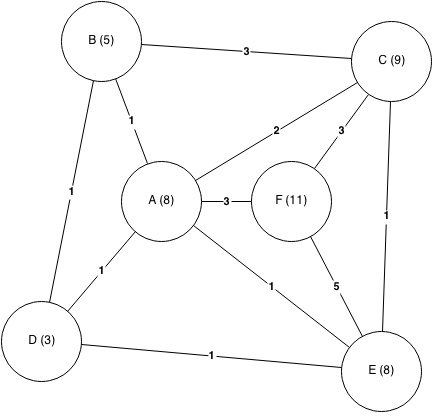
\includegraphics[width=\textwidth]{ejercicio-3-ejemplo-entrada.png}
		\caption{Grafo de entrada}
		\label{fig:ej3_ejemplo}
	\end{minipage}
	\begin{minipage}[t]{0.5\linewidth}
		\centering
		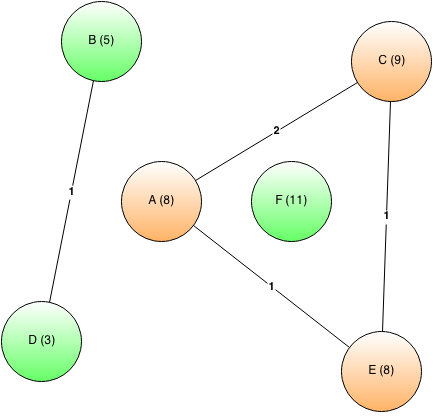
\includegraphics[width=\textwidth]{ejercicio-3-ejemplo-salida.png}
		\caption{La solución dada por la heurística, diferenciada con colores}
		\label{fig:ej3_ejemplo_solucion}
	\end{minipage}
\end{figure}

El problema de la heurística es que solamente compara el peso de un nodo con los conjuntos, sin tener en cuenta el resto de los nodos aún no asignados. Esto puede dar soluciones tan alejadas de la óptima como queramos. A saber:

Sea G un grafo cuyas aristas tienen peso 1, y k el parámetro de k-PMP. Es decir, el grado de un vértice es igual a su peso. G tiene dos tipos diferentes de nodos:
\begin{itemize}
    \item Los nodos $P_1, ..., P_k$ forman un subgrafo completo. Entonces, $d(P_i) = k-1$ en ese subgrafo.
    \item Los nodos $L_1, ..., L_N$ verifican que cada $L_i$ es solamente adyacente a todos los nodos $P_i$. Es decir, $d(L_i) = k$ para todo $i = 1, ..., N$.
\end{itemize}
Por lo anterior, los nodos $P_i$ tienen grado $N+k-1$. Estos nodos van a ser más pesados que los $L_i$ cuando $N > 1$, pues 
\begin{align*}
N+k-1 > k \Longleftrightarrow N > 1
\end{align*}
Supongamos entonces que hay más de un nodo de tipo $L$. Notemos además que el conjunto $\{L_1, ..., L_N\}$ tiene peso cero, ya que ningún par de nodos es adyacente entre sí.
Como el algoritmo ordena por peso de mayor a menor, el orden será del tipo 
\begin{align*}
[P_{i_1},...,P_{i_k},L_{j_1},...,L_{j_N}]
\end{align*}
Entonces, si N $>$ 1, el algoritmo va a elegir un nodo $P$ hasta que se terminen. A $P_{i_1}$ lo va a poner en $S_1$. A $P_{i_2}$ no lo puede poner en $S_1$ porque tiene peso 1 ahí (es adyacente a $P_{i_1}$, por lo tanto lo pone en $S_2$ que está vacío. A $P_{i_3}$ no puede ponerlo ni en $S_1$ ni en $S_2$ por la misma razón, entonces lo pone $S_3$. Así, una vez terminados todos los nodos $P$, la partición es
\begin{align*}
\{\{P_{i_1}\},\{P_{i_2}\},...,\{P_{i_k}\}\}
\end{align*}
Queda insertar los N nodos restantes, que son los $L_{j_1},...,L_{j_N}$. Pero para cualquiera de estos nodos, su peso en $S_x$ es 1 porque es adyacente a $P_{i_x}$. Como el algoritmo elige al primer conjunto y después chequea si eligiendo los demás mejora, y no lo hace en este caso, todos van a ir a $S_1$. Por lo tanto, la solución dada por el algoritmo será
\begin{align*}
\{ \{P_{i_1}, L_1, L_2, ..., L_N\}, \{P_{i_2}\}, ..., \{P_{i_k}\} \}
\end{align*}
El peso total de esta solución es N.
Pero si la solución fuera
\begin{align*}
\{ \{L_1, L_2, ..., L_N\}, \{P_{i_1}, P_{i_2}\}, ..., \{P_{i_k}\} \}
\end{align*}
el peso total sería 1. Es decir, la solución dada por la heurística golosa puede ser tan mala como queramos. Veamos gráficamente para k = 3 la diferencia:
\begin{figure}[H]
	\begin{minipage}[t]{\linewidth}
		\centering
		\frame{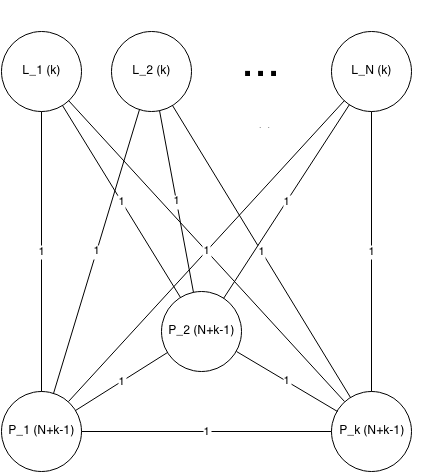
\includegraphics[width=0.5\textwidth]{ejercicio-3-rotura-heuristica.png}}
		\caption{Grafo de entrada}
		\label{fig:ej3_rotura_entrada}
	\end{minipage}
\end{figure}
\begin{figure}[H]
	\begin{minipage}[t]{0.5\linewidth}
		\centering
		\frame{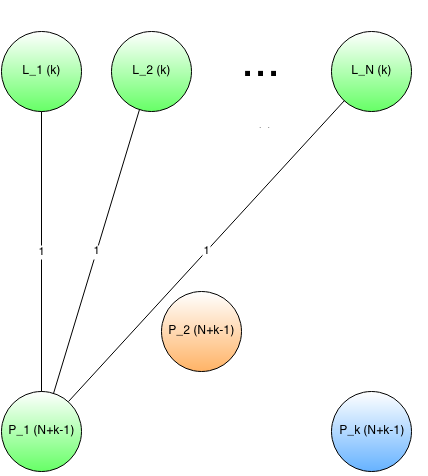
\includegraphics[width=\textwidth]{ejercicio-3-rotura-heuristica-solucion-golosa.png}}
		\caption{Solución golosa, con peso N.}
		\label{fig:ej3_rotura_golosa}
	\end{minipage}
	\begin{minipage}[t]{0.5\linewidth}
		\centering
		\frame{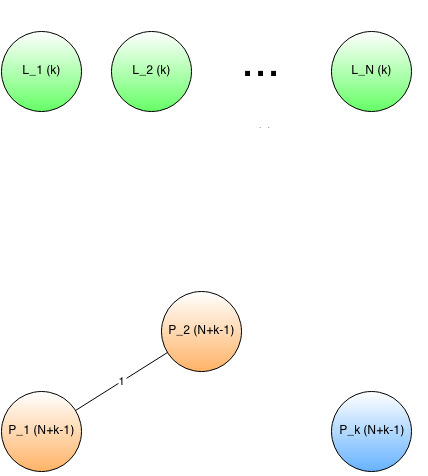
\includegraphics[width=\textwidth]{ejercicio-3-rotura-heuristica-solucion-optima.png}}
		\caption{Una solución óptima, con peso 1.}
		\label{fig:ej3_rotura_optima}
	\end{minipage}
\end{figure}

\subsection{Análisis de complejidad temporal}

Sea $n$ la cantidad de vértices del grafo de entrada, y $k$ el parámetro de k-PMP. Vamos a usar el pseudocódigo ya introducido para el cálculo de complejidad:
\begin{enumerate}
    \item En la primera línea se crean $k$ conjuntos vacíos. Esto cuesta $O(k)$. Llamaremos $C_i$ al i-ésimo conjunto.
    \item Luego, se crea un vector de tamaño $n$, con los vértices ordenados por peso en el grafo, de mayor a menor. Preguntarle a un vértice su peso en el grafo cuesta $O(n)$ porque representamos al grafo con una matriz de adyacencia, entonces en total es $O(n^2)$ saber el peso de todos los nodos. Finalmente, ordenar las tuplas $<nodo,peso(nodo)>$ cuesta $O(n \log n)$. Por lo tanto, todo esto cuesta $O(n^2)$. Al nodo i-ésimo de este nuevo ordenamiento lo llamaremos $u_i$.
    \item Ahora para cada $u_i$ se hace lo siguiente:
        \begin{enumerate}
            \item Inicializar las variables $pesoMinimo$ y $mejorConjunto$ cuesta $O(1)$.
            \item Para cada conjunto $C_i$ de la partición, se calcula el peso de $u_i$ en él y se chequea si es mejor para cambiar el $mejorConjunto$. El peso en un $C_i$ se calcula simplemente sumando los pesos de la aristas adyacentes entre $u_i$ y los vértices del conjunto, lo cual lleva $O(|C_i|)$. Sabemos que
            \begin{align*}
                \sum\limits_{\substack{i = 1}}^k |C_i| &= i - 1
            \end{align*}
            (pues sólo se asignaron $i - 1$ nodos en la iteración i-ésima). Por otro lado, estamos iterando sobre $k$ conjuntos, entonces el costo de este paso es $O(k) + O(i - 1)$.
            \item Insertar el nodo en $mejorConjunto$ cuesta $O(\log |mejorConjunto|)$ que podemos acotar por $O(\log (i - 1))$.
        \end{enumerate}
        En total, todo este paso cuesta
        \begin{align*}
                \sum\limits_{\substack{i = 1}}^n (O(k) + O(i-1) + O(\log (i - 1))) &= O(nk) + O(n^2) + O(\log n!)
        \end{align*}
        Por la aproximación de Stirling del factorial ($\log n! = n \log(n) - n + O(\log n)$), tenemos que $O(\log n!) = O(n \log n)$, entonces la complejidad total de este paso es $O(nk) + O(n^2)$.
\end{enumerate}
Tenemos entonces que la complejidad temporal de la heurística golosa es
\begin{align*}
    T(n,k) &= O(k) + O(n^2) + O(nk) + O(n^2) \\
    T(n,k) &= O(nk) + O(n^2)
\end{align*}
Como tomar valores $k \geq n$ no tiene sentido, ya que una solución óptima es trivial (se toma la partición $\{\{v_1\}, \{v_2\}, ..., \{v_n\}, \{\}, ..., \{\}\}$ que tiene peso total cero), entonces siendo $k < n$ vale que $O(nk) = O(n^2)$. Por lo tanto, la complejidad temporal de peor caso de la heurística para un tamaño de entrada de $n$ vértices es
\begin{align*}
    T(n) &= O(n^2)
\end{align*}


\newpage
% Bibliografía
%\addcontentsline{toc}{section}{Referencias}
\begin{thebibliography}{11}

\bibitem{cormen}
  Thomas H. Cormen,
  \emph{Introduction to Algorithms}.
  The MIT Press, Massachusetts,
  3rd edition,
  2009.

\end{thebibliography}
%\bibliographystyle{plain}
%\bibliography{referencias}

\end{document}
